\documentclass[11pt,twoside,final
]{article}
\usepackage{amsmath,amsfonts,amssymb,amsthm,indentfirst,enumerate,textcomp}
\usepackage[utf8]{inputenc}
\usepackage{chebsb}
\usepackage[russian]{babel}
\usepackage{indentfirst, array}
\usepackage{amscd,latexsym}
\usepackage{mathrsfs}
%\usepackage[ruled, linesnumbered]{algorithm2e}
\usepackage{tabularx}
\usepackage{multirow}

\usepackage{graphicx}
\usepackage{textcase}% Оформление страниц

\graphicspath{ {./img/} }

\label{beg}
% заглавие стати и аннотация

\levkolonttl{%левый колонтитул - авторы
И.~Б.~Кожухов, А.~М.~Пряничников}
\prvkolonttl{%правый колонтитул - сокращенное название статьи
Об унарах с тождествами в решётке конгруэнций, II}

\newcommand{\god}{2025} % Для подавления ошибки при компиляции проекта

\UDK{% УДК статьи
512.567.5 + 512.579}

\DOI{
10.22405/2226-8383-\god-\tom-\iss-\pageref{beg}-\pageref{end}
}

\title
{%название статьи на русском языке с указанием источника финансирования при необходимости
Об унарах с тождествами в решётке конгруэнций, II}
{%название статьи на английском языке
On unars with identities in congruence lattice, II}

\author
{%авторы статьи
И. Б. Кожухов, А. М. Пряничников}
{%авторы статьи
I. B. Kozhukhov, A. M. Pryanichnikov}

\Cite{
И. Б. Кожухов, А. М. Пряничников. Об унарах с тождествами в решётке конгруэнций, II // Чебышевcкий сборник, \god, т.~\tom, вып.~\iss, с.~\pageref{beg}--\pageref{end}.
}
{Kozhukhov, I. B., Pryanichnikov, A. M. \god, ``On unars with identities in congruence lattice, II''\,, {\it Che\-by\-shev\-skii sbornik}, vol.~\tom, no.~\iss, pp.~\pageref{beg}--\pageref{end}.
}

\info
{%авторы статьи на русском языке
\noindent {\bf Кожухов Игорь Борисович}~--- д.ф.-м.н., Нац. исслед. университет МИЭТ; механико-математический факультет МГУ; Гос. академия нар. хоз-ва и гос. службы (г. Москва).

\noindent
\emph{e-mail: kozhuhov\_i\_b@mail.ru}

\noindent {\bf Пряничников Алексей Михайлович}~--- механико-математический факультет МГУ, ООО <<Квантом>> (г. Москва).

\noindent
\emph{e-mail: genary@ya.ru}


}
{%авторы статьи на английском языке
\noindent {\bf Kozhukhov Igor Borisovich}~--- Dr. Phys.-Math. Sci., Nat. Res. Univ. MIET; Fac. of Mech. and Math. of Moscow State Univ.; Russian Presidental Academy of Nat. Econom. and Public Admin., (Moscow).

\noindent
\emph{e-mail: kozhuhov\_i\_b@mail.ru}

\noindent {\bf Pryanichnikov Alexey Mikhailovich}~--- Fac. of Mech. and Math. of Moscow State Univ., <<Kvantom>> LLC, (Moscow).

\noindent
\emph{e-mail: genary@ya.ru}

}

\Abstract
{%Аннотация статьи на русском языке 150-250 слов с учетом ключевых слов
В статье доказано, что если решётка конгруэнций унара удовлетворяет нетривиальному решёточному тождеству, то унар является гомоморфным образом копроизведения конечного числа прямых и лучей.
}
{%Аннотация статьи на английском языке
In paper we prove that if a congruence lattice of an unar holds a nontrivial lattice identity, then the unar is a homomorphic image of a coproduct of finite numbers of lines and rays.
}

\keywords
{%ключевые слова на русском языке
полигон над полугруппой, унар, решётка конгруэнций, тождество.
}
{%ключевые слова на английском языке
act over semigroup, unar, congruence lattice, identity.
}

%число наименований в библиографии
\Bibliography{14 названий.}{14 titles.}

\def\Con{\operatorname{Con}}
\def\Eq{\operatorname{Eq}}
\def\indeg{\operatorname{indeg}}
\def\outdeg{\operatorname{outdeg}}
\def\ind{\operatorname{ind}}

\begin{document}

%генерация заглавия статьи
\maketitle

\enmaketitle

\section{Введение}

Решётка конгруэнций $\Con \mathbf{A}$ универсальной алгебры $\mathbf{A}$ — важная характеристика этой алгебры.
Это полная решётка с наименьшим элементом $\Delta = \{ (a,a) \mid a \in \mathbf{A} \}$ и наибольшим элементом $\nabla = \mathbf{A} \times \mathbf{A}$, причём $\Con \mathbf{A}$ является полной подрешёткой решётки $\Eq \mathbf{A}$ всех отношений эквивалентности на множестве $\mathbf{A}$.
Изучение алгебр с условиями на решётку конгруэнций — активно развивающееся и богатое содержанием направление общей алгебры.
Сюда относятся условия максимальности и минимальности, приводящие к понятиям артиновых и нётеровых алгебр, условие простоты (когда $\Con \mathbf{A} = \{ \Delta, \nabla \}$), антипростоты ($\Con \mathbf{A} = \Eq \mathbf{A}$), дистрибутивности или модулярности (т.е. решётка $\Con \mathbf{A}$ дистрибутивна или модулярна), подпрямой неразложимости и т.д.

Алгебрам $\mathbf{A}$, у которых решётка конгруэнций $\Con \mathbf{A}$ является дистрибутивной или модулярной, посвящено значительное число работ разных авторов. 
Дистрибутивные и модулярные полигоны над полугруппами изучались в~\cite{Ptakhov_2}, полное описание таких полигонов над полугруппами левых или правых нулей получено в~\cite{Khaliullina_3}. 
В работе~\cite{Egorova_4} были описаны дистрибутивные и модулярные унары.
Дистрибутивность решётки $\Con \mathbf{A}$ означает выполнение в ней тождества $ (x \vee y) \wedge z = (x \wedge z) \vee (y \wedge z) $, модулярность задаётся тождеством $ (x \vee y) \wedge (x \vee z) = x \vee (z \wedge (x \vee y)) $.
Естественным представляется изучение алгебр $\mathbf{A}$, у которых решётка $\Con \mathbf{A}$ удовлетворяет какому-нибудь нетривиальному решёточному тождеству.
Данное условие является \textit{условием конечности}, так как любая конечная алгебра ему удовлетворяет (это следует из того, что всякая конечная решётка удовлетворяет нетривиальному тождеству — см. лемму 3).
Многообразия алгебр, у которых решётки конгруэнций всех алгебр удовлетворяют одному и тому же нетривиальному тождеству, посвящены монография~\cite{Kearnes_5} и диссертация~\cite{Nation_6}.
В работе~\cite{Repnitsky_7} были описаны коммутативные полугруппы, у которых решётки подполугрупп удовлетворяют нетривиальному решёточному тождеству.
Цель данной работы — найти необходимое условие того, что решётка конгруэнций унара (полигона над свободной циклической полугруппой) удовлетворяет нетривиальному тождеству.
Является ли это условие достаточным, авторам неизвестно.

Работа является продолжением работы~\cite{Kozhukhov_8}.
Основные определения мы здесь приведём, за доказательствами отошлём читателя к работе~\cite{Kozhukhov_8}.
Отметим, что заключительное утверждение, сформулированное в последнем абзаце работы~\cite{Kozhukhov_8}, требует корректировки: вместо «копроизведения конечного числа прямых» следовало написать «копроизведения конечного числа прямых и лучей».

Основные сведения из универсальной алгебры можно найти в~\cite{Kohn_9}, из теории решёток — в~\cite{Gretzer_10}, теории полугрупп — в~\cite{Clifford_11}, полигонов над полугруппами — в~\cite{Kilp_1}, унаров — в~\cite{Jakubikova_12}, многообразий решёток — в~\cite{Jipsen_13}.


\section{Основные определения}

\textit{Полигон над полугруппой} — это множество $X$, на котором действует полугруппа $S$, т.е. определено отображение $X \times S \to X$, $(x,s) \mapsto xs$ удовлетворяющее условию $x(st) = (xs)t$ при $x \in X$, $s,t \in S$ (см.~\cite{Kilp_1}).
Полигон над полугруппой является алгебраической моделью \textit{автомата}.
Кроме того, понятие полигона фактически совпадает с понятием \textit{унарной алгебры}.

Подмножество $Y \subseteq X$ называется \textit{подполигоном}, если $YS \subseteq Y$.
Элемент $z \in X$ называется \textit{нулём}, если $zs = z$ при всех $s \in S$.
Нулей у полигона, в отличие от полугруппы, может быть сколько угодно (в полугруппе нуль, если он существует, единственен).
\textit{Решётку конгруэнций} полигона $X$ над полугруппой $S$ мы будем обозначать $\Con_S X$ или просто $\Con X$.

Пусть $X$ — полигон над полугруппой $S$ и $Y$ — его подполигон.
Положим $ \rho_Y = (Y \times Y) \cup \Delta_X $.
Это конгруэнция полигона $X$, называемая \textit{конгруэнцией Риса}, соответствующей подполигону $Y$.
Нетрудно видеть, что для любого подполигона $Y$, у конгруэнции Риса $\rho_Y$ один из классов есть множество $Y$, а другие классы одноэлементны.
Для фактор-полигона $X/\rho_Y$ мы будем также использовать краткую запись: $X/Y$.

Пусть $X$ — полигон над полугруппой $S$ и $X_i$ ($i \in I$) — его подполигоны, причём $X = \bigcup_{i \in I} X_{i}$ и $X_{i} \cap X_{j} = \varnothing$ при $i \neq j$.
В этом случае мы называем полигон $X$ \textit{копроизведением} полигонов $X_i$ и пишем $X = \bigsqcup_{i \in I} X_{i}$.
В работах по унарам копроизведение называют обычно прямой суммой.

Для полугруппы $S$ полагаем $S^1 = S \cup \{ 1 \}$.
Здесь $S^1$ — полугруппа, полученная присоединением к $S$ внешним образом единицы (при этом считаем, что $s \cdot 1 = 1 \cdot s = s$ для каждого $s \in S^1$).
Если $X$ — полигон над $S$, то его можно сделать полигоном над полугруппой $S^1$, положив $x \cdot 1 = x$ при $x \in X$.

На полигоне $X$ над полугруппой $S$ можно ввести отношение \textit{квазипорядка} $\leqslant$ (рефлексивное и транзитивное отношение), полагая $x \leqslant y \Leftrightarrow x \in yS^1$.
Полигон $X$ называется \textit{связным}, если для любых $x,y \in X$ существуют элементы $x_1,\ldots,x_{2n} \in X$ такие, что  $ x \leqslant x_1 \geqslant x_2 \leqslant \ldots \geqslant x_{2n} \leqslant y$.
Нетрудно видеть, что любой полигон $X$ является копроизведением связных подполигонов $X_i$ (\textit{компонент связности}).

\textit{Унар}, т.е. множество $X$ с одной унарной операцией $f: X \to X$, можно рассматривать как полигон над свободной циклической полугруппой $S = \{ a,a^{2},a^{3},\ldots\}$, при этом $x \cdot a = f(x)$ для $x \in X$.

Для унара $X$ и элемента $x \in X$ полагаем $xS = \{ xa^k \mid k \geqslant 1 \}$, $xS^{-1} = \{ y \mid \exists k \geqslant 1 \ y a^k = x \}$, $xa^{-1} = \{ y \mid ya = x \}$.

Также нам понядобятся некоторые понятия из теории графов.
В ориентированном графе $G$ с множеством вершин $V(G)$ и рёбер $E(G)$ для каждой вершины $x \in V(G)$ определяются понятия \textit{входной степени}
\[
	\indeg x = |\{ y \mid (y,x) \in E(G) \}|
\]
и \textit{выходной степени}
\[
	\outdeg x = |\{ y \mid (x,y) \in E(G) \}|
\]
вершины $x$.
Понятно, что у унара $X$, рассматриваемого как граф, $\outdeg x = 1$ и $\indeg x = |xa^{-1}|$ для всех $x \in X$.

Пусть $X$ -- унар и $x,y \in X$. Если $y = x a^k$ при некотором $k \geqslant 0$, причём $k$ -- наименьшее среди таких $l \geqslant 0$, что $x a^l = y$, то число $k$ назовём \textit{индексом элемента} $y$ относительно $x$ и обозначим $\ind_x y$: $$ \ind_x y = \min \{ k \geqslant 0 \mid xa^k = y \}. $$

Пусть $X$-- унар.
Элемент $x \in X$ назовём \textit{узлом}, если существуют элементы $y,z \in X$ такие, что $y \neq z$ и $y \cdot a = z \cdot a = x$.
Приведённое здесь определение узла отличается от приведённого в~\cite{Kozhukhov_8}.
Элемент $x \in X$ \textit{периодический}, если $x \cdot a^n = x$ для некоторого $n > 0$.
Элементы $x \in X \setminus XS$ будем называть \textit{начальными}.
\textit{Прямой} называется унар, изоморфный унару $\mathbb{Z}$ с операцией $i \cdot a = i + 1$ при $i \in \mathbb{Z}$ (см. рисунок~\ref{fig:line}).
\begin{figure}[ht!]
	\centering
	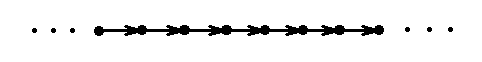
\includegraphics[scale=0.6]{img/line.png}
	\caption{Прямая (унар).}
	\label{fig:line}
\end{figure}

\textit{Лучом} называется унар, изоморфный унару $\mathbb{N}$ с операцией $i \cdot a = i + 1$ при $i \in \mathbb{N}$ (см. рисунок~\ref{fig:ray}).
\begin{figure}[ht!]
	\centering
	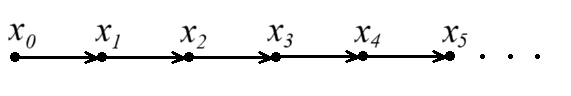
\includegraphics[scale=0.5]{img/ray.png}
	\caption{Луч (унар).}
	\label{fig:ray}
\end{figure}

Основным результатом работы является следующее утверждение.
\begin{theorem} \label{thm:main}
	Если решётка конгруэнций унара удовлетворяет нетривиальному решёточному тождеству, то унар является гомоморфным образом копроизведения конечного числа прямых и лучей.
\end{theorem}

Доказательство теоремы основывается на ряде вспомогательных утверждений, часть из которых верны не только для унаров, но и для более широкого класса полигонов.
\begin{lemma}[{\cite[лемма 1]{Kozhukhov_8}}] \label{lemma:1}
	Если $X$ — полигон над полугруппой $S$, $Y$ — его подполигон и $\rho_Y$ — конгруэнция Риса, то решётки $\Con Y$ и $\Con (X/Y)$ изоморфно вкладываются в решётку $\Con X$.
\end{lemma}

Для дальнейшего нам понадобится несколько фактов из теории многообразий решёток.
Решёточное тождество $p = q$ называется \textit{нетривиальным}, если оно выполняется не во всех решётках, но выполняется в какой-либо нетривиальной решётке (т.е. отличной от $\{\nabla,\ \Delta\}$).
Здесь $p,q$ — термы сигнатуры $\{ \land , \lor \}$.

\begin{lemma}[{\cite[лемма 2]{Burris_14}}] \label{lemma:2}
	Решётка $\Eq A$, где $A$ -- бесконечное множество, не удовлетворяет никакому нетривиальному тождеству.
\end{lemma}

Следующее утверждение известно, его доказательство можно получить на основании~\cite[следствие 3.14 и теорема 8 главы VI]{Kohn_9}.
\begin{lemma}\label{lemma:3}
	Всякая конечная решётка удовлетворяет некоторому нетривиальному тождеству.
\end{lemma}

\begin{lemma}[{\cite[леммы 4,5,6]{Kozhukhov_8}}] \label{lemma:4}
	Пусть $X$ — полигон над полугруппой $S$.
	Если решётка $\Con X$ удовлетворяет нетривиальному тождеству, то:
	\begin{enumerate}
		\item $X$ имеет лишь конечное число компонент связности;
		\item множество $X \setminus XS$ конечно (т.е. количество начальных элементов конечно);
		\item $X$ имеет лишь конечное число периодических элементов;
		\item $X$ не содержит бесконечного множества попарно несравнимых относительно естественного квазипорядка элементов.
	\end{enumerate}
\end{lemma}

\section{Основная часть}

\begin{lemma} \label{lemma:5}
	Если решётка $\Con X$ унара $X$ удовлетворяет нетривиальному тождеству, то $\indeg x < \infty$ для каждого $x \in X$.
\end{lemma}
\begin{proof}
	Предположим, что утверждение леммы неверно, т.е. множество $xa^{-1}$ бесконечно при некотором $x \in X$.
	Отсюда следует, что можно найти различные элементы $y_1, y_2, \ldots \in X $ такие, что $y_n a = x$ при всех $n \in \mathbb{N}$.
	Рассмотрим унар $Y = \bigcup_{n \in \mathbb{N}} y_n S$ и фактор-унар $\overline{Y} = Y / x S^1$.
	Так как решётка $\Con X$ удовлетворяет нетривиальному тождеству, то по лемме~\ref{lemma:1} решётка $\Con \overline{Y}$ удовлетворяет тому же тождеству.
	Но это невозможно, так как унар $Y$ является унаром с нулевым умножением, а значит, $\Con \overline{Y} = \Eq \overline{Y}$, что противоречит лемме~\ref{lemma:2} ввиду того, что множество $\overline{Y}$ бесконечно.
\end{proof}

\begin{lemma} \label{lemma:6}
	Пусть $X$ -- связный унар, у которого решётка $\Con X$ удовлетворяет нетривиальному тождеству.
	Пусть $u_0$ -- узел такой, что элементы $u_0 a, u_0 a^2, \ldots$ различны и не являются узлами.
	Если унар $X$ имеет бесконечно много узлов, то существуют элементы $u_{-1}, u_{-2}, \ldots$ такие, что $u_i a = u_{i + 1}$ при всех $i \in \mathbb{Z}$ и в подунаре $\{ u_i \mid i \in \mathbb{Z} \}$ бесконечно много узлов.
\end{lemma}
\begin{proof}
	По лемме~\ref{lemma:5} множество $u_0 a^{-1}$ конечно.
	Пусть $u_0 a^{-1} = \{ x_1, \ldots, x_m \}$.
	Так как $X$ связен и элементы $u_0 a, u_0 a^2, \ldots$ не являются узлами, то $X = u_0 S^1 \cup \bigcup_{i=1}^m (\{ x_i \} \cup x_i S^{-1})$.
	Так как узлов в $X$ бесконечно много, а в $u_0 S^1$ их конечное число (1 штука), то в каком-либо из множеств $\{ x_i \} \cup x_i S^{-1}$ бесконечно много узлов унара $X$.
	Без ограничения общности можно считать, что в множестве $x_1 S^{-1}$ бесконечно много узлов.
	Если $x_1$ -- узел, то положим $y_{-1} = x_1$ и перейдём к множеству $y_{-1} a^{-1}$, поступая с ним так же, как и с множеством $u_0 a^{-1}$.
	Если $x_1$ -- не узел, то множество $x_1 a^{-1}$ состоит из одного элемента.
	Если этот элемент не узел, то перейдём к элементу $x_1 a^{-2}$ и т.д.
	Так как такой <<подъём>> по этой цепочке бесконечно идти не может, то в результате получим узел, обозначим его через $y_{-1}$.
	Итак, $y_{-1}$ -- узел такой, что $y_{-1} a^t = u_0$ при некотором $t \geqslant 1$, а $y_{-1} a^s$ не является узлом при $0 < s < t$.
	Далее, с узлом $y_{-1}$ поступаем так же, как и с $u_0$.
	И так далее.
	Получим последовательность узлов $y_{-1}, y_{-2}, \ldots$.
	Подунар, порождённый элементами $y_{-1}, y_{-2}, \ldots$ -- искомый.
\end{proof}

\begin{lemma} \label{lemma:7}
	Если решётка $\Con X$ унара $X$ удовлетворяет нетривиальному тождеству, то $X$ имеет лишь конечное число узлов.
\end{lemma}
\begin{proof}
	Нетрудно увидеть, что все узлы делятся на два типа (см. рисунок 4): где $x \notin \{ y, z \}$ и где $x \in \{ y, z \}$.
	\begin{figure}[ht!]
		\centering
		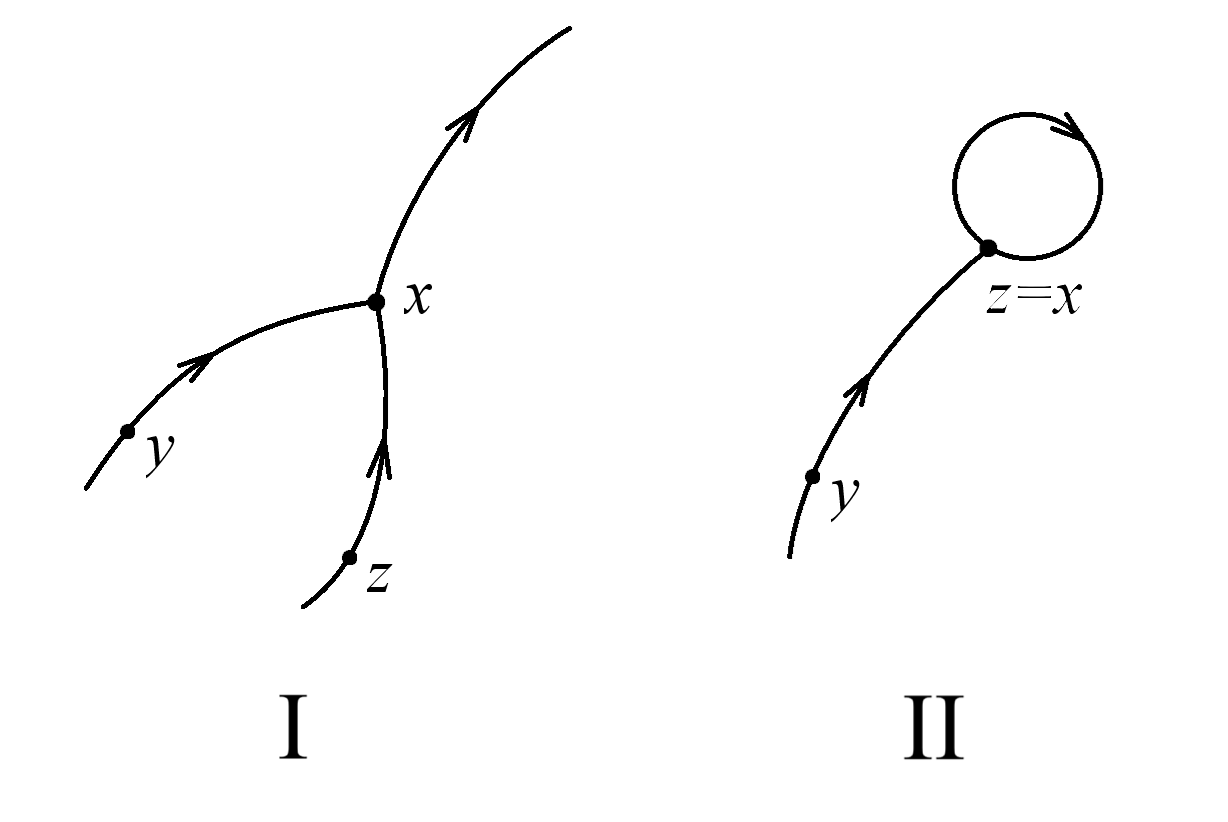
\includegraphics[scale=0.4]{img/uzly.png}
		\caption{Типы узлов.}
		\label{fig:uzly}
	\end{figure}
	Очевидно, что узлов второго типа в одной компоненте связности может быть не более одного (см. утверждение (3) леммы~\ref{lemma:4}).
	Так как по утверждению (1) леммы~\ref{lemma:4} компонент связности конечное число, то и число таких узлов тоже конечно.
	
	Осталось показать, что узлов первого типа конечное число.
	Пусть это не так, т.е. их бесконечно много.
	Так как по утверждению (1) леммы~\ref{lemma:4} число компонент связности конечно, то узлов первого типа бесконечно много в какой-либо компоненте.
	Рассмотрим эту компоненту связности (обозначим её через $Y$), возьмём в ней какой-нибудь узел $u_{1}$ и разберём два случая.
	
	\textit{Случай 1}: среди элементов $u_{1}a,u_{1}a^{2},u_{1}a^{3},\ldots$ бесконечно много узлов.
	Тогда имеем: $u_{1},u_{1}a^{i_{1}},u_{1}a^{i_{2}},\ldots$ — узлы, $0 < i_{1} < i_{2} < \ldots$ (см. рисунок~\ref{fig:uzly_2}).
	\begin{figure}[ht!]
		\centering
		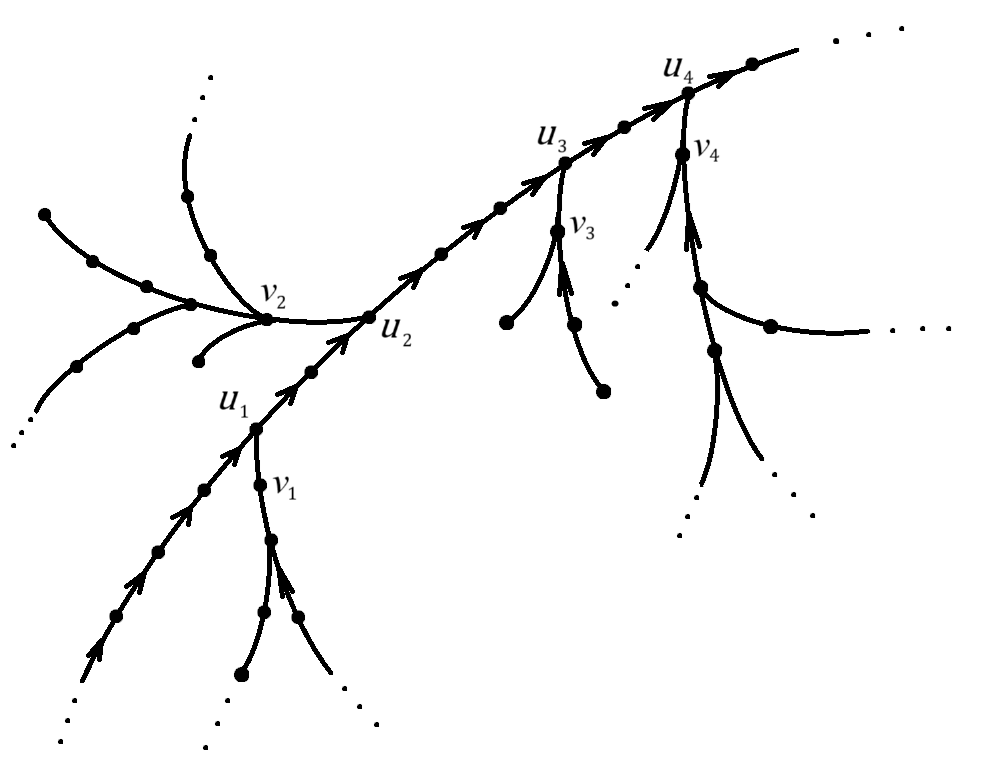
\includegraphics[scale=0.8]{img/uzly_2.png}
		\caption{Узлы $u_i$ в компоненте связности $Y$.}
		\label{fig:uzly_2}
	\end{figure}
	
	Пусть $v_k a = u_k$ ($k = 1,2,\ldots$).
	Обозначим через $Y$ компоненту связности, содержащую $u_{1}$.
	Удалим из рассмотрения те $u_{i}$, для которых существует начальный элемент $x$ и число $k \geqslant 0$, для которых $x a^{k} = v_i$.
	Так как по лемме~\ref{lemma:4}(2) начальных элементов лишь конечное число, то удалено будет лишь конечное число узлов $u_{i}$.
	Из изображённых на рисунке~\ref{fig:uzly_2}, удалёнными будут узлы $u_2$ и $u_3$.
	Перенумеруем оставшиеся узлы $u_i$ так, чтобы $v_i \notin (X \setminus XS)S^{1}$ при $i = 1,2,\ldots$.
	
	Рассмотрим подунар $Y' = u_1 S^1$ унара $Y$ и фактор-унар $\overline{Y} = Y/Y'$ (см. рисунок~\ref{fig:uzly_3}).
	Нуль унара $\overline{Y}$ обобзначим через $z$.
	\begin{figure}[ht!]
		\centering
		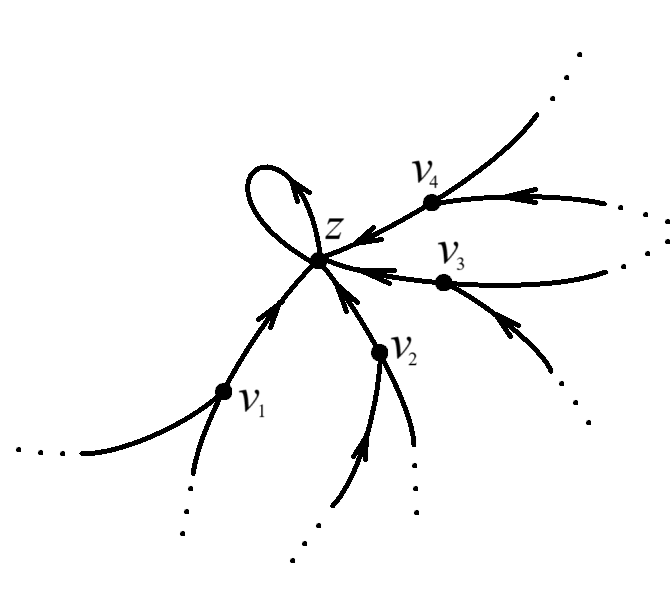
\includegraphics[scale=0.7]{img/uzly_3.png}
		\caption{Фактор-унар $\overline{Y}$.}
		\label{fig:uzly_3}
	\end{figure}
	Так как $v_i \notin Y'$ при всех $i \in \mathbb{N}$, то элементы $v_i$ различны в унаре $\overline{Y}$.
	Так как решётка $\Con X$ удовлетворяет нетривиальному тождеству, то по лемме~\ref{lemma:1} решётка $\Con \overline{Y}$ удовлетворяет этому же тождеству.
	Так как $v_i a = z$ при всех $i \in \mathbb{N}$ и $v_i$ различны, то $\indeg z = \infty$, а это противоречит лемме~\ref{lemma:5}.
	
	\textit{Случай 2}: среди элементов $u_{1}a,u_{1}a^{2},u_{1}a^{3},\ldots$ лишь конечное число узлов унара $X$.
	Здесь возможны две ситуации: либо последовательность $u_1, u_1 a, u_1 a^2, \ldots$ заканчивается циклом длины $m$: $\{ u_1 a^r, u_1 a^{r + 1}, \ldots, u_1 a^{r + m - 1} \}$ $(u_1 a^{r + m} = u_1 a^r)$, либо элементы $u_1, u_1 a, u_1 a^2, \ldots$ различны, и тогда есть последний узел $u_1 a^k$, т.е. такой узел, что элементы $u_1 a^t$ при $t > k$ не являются узлами.
	И в той, и в другой ситуации мы имеем, что все узлы унара $Y$ лежат в множестве $\{ y_0 \} \cup y_0 S^{-1}$ для некоторого $y_0 \in Y$, который можно считать узлом.
	По лемме~\ref{lemma:5} множество $y_0 a^{-1}$ конечно.
	Пусть $y_0 a^{-1} = \{ x_1, \ldots, x_m \}$.
	Очевидно, в каком-либо из множеств $x_i S^{-1}$ лежит бесконечно много узлов.
	Можно считать, что множество $x_1 S^{-1}$ содержит бесконечно много узлов.
	Если $x_1$ -- узел, то положим $y_1 = x_1$ и перейдём к множеству $y_1 a^{-1}$, поступая с ним так же, как с множеством $y_0 a^{-1}$.
	Если же $x_1$ -- не узел, то множество $x_1 a^{-1}$ состоит из одного элемента.
	Так как $x_1 S^{-1} = \{ x_1 \} \cup x_1 a^{-1} \cup x_1 a^{-1} S^{-1} $, а значит, при каком-то $t$ мы получим узел $x_1 a^{-t}$, причём можно считать, что элементы $x_1, x_1 a^{-1}, \ldots, x_1 a^{-(t-1)}$ не являются узлами.
	Положим $y_1 = x_1 a^{-t}$ и поступим с элементом $y_1$ так же, как поступили с элементом $y_0$.
	Продолжая этот процесс, мы получим узлы $y_1,y_2,\ldots$ такие, что $y_k a^{j_k} = y_{k - 1}$ при подходящих $j_k > 0$ $(k = 1,2,\ldots)$.
	Так как $y_k$ -- узлы, то существуют $z_k \in Y$ такие, что $z_k a = y_k$ и $z_k \notin y_{k + 1}S$ (см. рисунок~\ref{fig:uzly_4}).
	\begin{figure}[ht!]
		\centering
		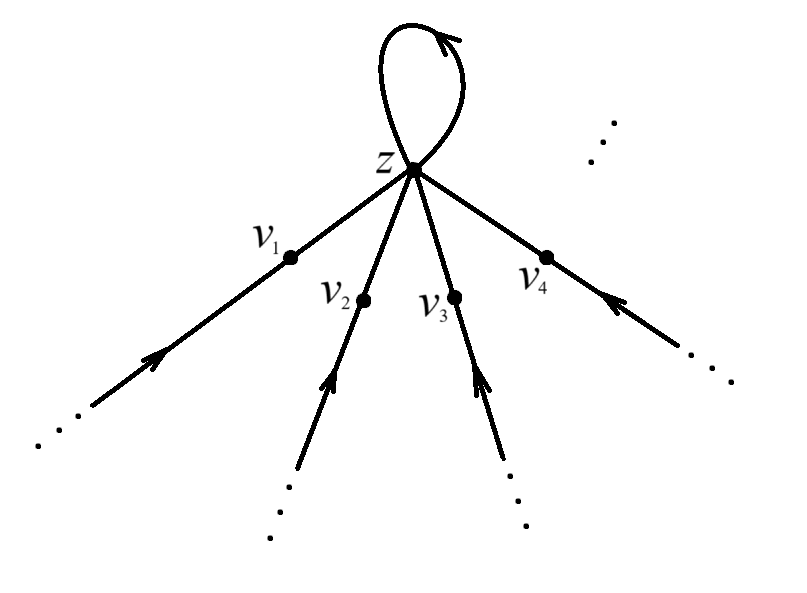
\includegraphics[scale=0.6]{img/uzly_4.png}
		\caption{Узлы $y_0, y_1, y_2, \ldots$.}
		\label{fig:uzly_4}
	\end{figure}
	Пусть $Y' = \bigcup_{k=1}^{\infty} y_k S$ и $\overline{Y} = Y / Y'$.
	По лемме~\ref{lemma:1} решётка $\Con \overline{Y}$ удовлетворяет нетривиальному тождеству.
	Однако, в унаре $\overline{Y}$ выполняется равенство $z_k a = 0$ при всех $k \in \mathbb{N}$, где $0$ обозначает нулевой элемент унара $\overline{Y}$.
	Поэтому $\indeg 0 = \infty$, а это противоречит лемме~\ref{lemma:5}.
\end{proof}



\section{Заключение}

%библиография по ГОСТу
\begin{thebibliography}{99}
	
	\bibitem{Kilp_1}
	Kilp~M., Knauer~U., Mikhalev~A.\,V. Monoids, acts and categories // Berlin - N.Y., de Gruyter, 2000. 529 P.
	
	\bibitem{Ptakhov_2}
	Птахов~Д.\,О., Степанова~А.\,А. Решётки конгруэнций полигонов // Дальневост. матем. журн. 2013. Т.~13, №1. С.~107--115.
	
	\bibitem{Khaliullina_3}
	Халиуллина~А.\,Р. Условия модулярности решётки конгруэнций полигона над полугруппой правых или левых нулей // Дальневост. матем. журн. 2015. Т.~15, №~1. С.~102--120.
	
	\bibitem{Egorova_4}
	Егорова~Д.\,П. Структура конгруэнций унарной алгебры // Межвузовский научный сборник «Упорядоченные множества и решётки». г. Саратов: Издательство Саратовского университа. 1978. Вып.~5. С.~11--43.
	
	\bibitem{Kearnes_5}
	Kearnes~K.\,A., Kiss~E.\,W. The shape of congruence lattices // Memoirs of the American Mathematical Society. 2013. Vol.~222. 169 P.
	
	\bibitem{Nation_6}
	Nation~J.\,B. Varieties of algebras whose congruence lattices satisfy lattice identities (Thesis) // Pasadena: California Institute of Technology. 1973. 63 P.
	
	\bibitem{Repnitsky_7}
	Репницкий~В.\,Б., Кацман~С.\,И. Коммутативные полугруппы, решётка подполугрупп которых удовлетворяет нетривиальному тождеству // Математический сборник. 1988. Т.~137(179), №~4(12). С.~462--482.
	
	\bibitem{Kozhukhov_8}
	Кожухов~И.\,Б., Пряничников~А.\,М. Об унарах с тождествами в решётке конгруэнций // Материалы VI международной научно-технической конференции СИТОНИ-2019. Донецк, 2019. С.~64--69.
	
	\bibitem{Kohn_9}
	Кон~П.\,М. Универсальная алгебра // М.: Мир, 1968. 359~С.
	
	\bibitem{Gretzer_10}
	Гретцер~Г. Общая теория решёток // М.: Мир, 1982. 454~С.
	
	\bibitem{Clifford_11}
	Клиффорд~А., Престон~Г. Алгебраическая теория полугрупп // М.: Мир, 1972. Т.~1. 286~с.; Т.~2. 423~С.
	
	\bibitem{Jakubikova_12}
	Jakubiková-Studenovská~D., Pócs~J. Monounary algebras // Košice: UPJS, 2009. 301~P.
	
	\bibitem{Jipsen_13}
	Jipsen~P., Rose~H. Variety of lattices // Lecture Notes in Mathematics, 1992. Vol.~1533. 166~P.
	
	\bibitem{Burris_14}
	Burris~S., Sankappanavar~H.\,P. A course in universal algebra // Springer New York, 1981, Vol.~78, 276~P.
	
\end{thebibliography}


%библиография по Гарвардскому стандарту
\begin{engbibliography}{99}
	
	\bibitem{en_Kilp_1}
	Kilp, M., Knauer, U. \& Mikhalev, A.\,V. 2000, ``Monoids, acts and categories``, \textit{Berlin; New York: de Gruyter}, 546 pp.
	
	\bibitem{en_Ptakhov_2}
	Ptahov, D.\,O. Stepanova, A.\,A. 2013, ``Congruence lattice of S-acts``, \textit{Far Eastern Mathematical Journal}, vol. 13, no. 1, pp. 107--115.
	
	\bibitem{en_Khaliullina_3}
	Khaliullina, A.R. 2015, ``Modularity conditions of the lattice of congruences of acts over right or left zero semigroups``, \textit{Far Eastern Mathematical Journal}, vol. 15, no. 1, pp. 102--120.
	
	\bibitem{en_Egorova_4}
	Egorova, D.\,P. 1978, ``The structure of congruences of unary algebra``, \textit{Interuniversity scientific collection "Ordered sets and lattices"}, Saratov: Saratov University Press, issue 5, pp. 11--4. (in Russian)
	
	\bibitem{en_Kearnes_5}
	Kearnes, K.\,A., Kiss, E.\,W. 2013, ``The shape of congruence lattices``, \textit{Memoirs of the American Mathematical Society}, vol. 222, 169 pp.
	
	\bibitem{en_Nation_6}
	Nation, J.\,B. 1973, ``Varieties of algebras whose congruence lattices satisfy lattice identities``, \textit{PhD thesis, California Institute of Technology}, 63 pp.
	
	\bibitem{en_Repnitsky_7}
	Repnitsky, V.\,B., Katsman, S.\,I. 1990, ``Commutative semigroups with lattice of subsemigroups satisfies a nontrivial identity``, \textit{Mathematics of the USSR-Sbornik}, vol. 65, no. 2, pp. 465--485.
	
	\bibitem{en_Kozhukhov_8}
	Kozhukhov, I.\,B., Pryanichnikov, A.\,M. 2019, ``On unars with identities in congruence lattice``', \textit{Proceedings of the VI International Scientific and Technical Conference SITONI-2019}, Donetsk, pp. 64--69. (in Russian)
	
	\bibitem{en_Kohn_9}
	Kohn, P.\,M. 1981, ``Universal algebra``, \textit{Springer Dordrecht}, 412 pp.
	
	\bibitem{en_Gretzer_10}
	Grätzer, G. 2011, \textit{Lattice Theory: Foundation}, Birkhäuser Basel, 614 pp.
	
	\bibitem{en_Clifford_11}
	Clifford, A.\,H., Preston, G.\,B. 1961--1967, ``The algebraic theory of semigroups``, \textit{American Mathematical Society. Mathematical Surveys}, Providence, Rhode Island, no. 7, vol. I-II, 244 pp. and 350 pp.
	
	\bibitem{en_Jakubikova_12}
	Jakubiková-Studenovská, D., Pócs, J. 2009, ``Monounary algebras``, \textit{UPJS}, Košice, 301 pp.
	
	\bibitem{en_Jipsen_13}
	Jipsen, P., Rose, H. 1992, Variety of lattices, \textit{Lecture Notes in Mathematics}, Springer Berlin, vol. 1533, 166 pp.
	
	\bibitem{en_Burris_14}
	Burris, S., Sankappanavar, H.P. 1981, A course in universal algebra, \textit{Springer New York}, vol. 78, 276 pp.
	
\end{engbibliography}

\label{end}

\end{document}